%!TeX spellcheck = en-US
%!TEX root = ../hw1_report.tex
As can be seen from Figure \ref{fig:task2} the rate of convergence is linear for the power method, as expected. For the Rayleigh quotient iteration the rate of convergence is cubic when $A$ is symmetric and quadratic when $A$ is nonsymmetric. This is also expected. The rate of convergence $p$ for the respective settings is approximated to $p\approx 3.03$ and $p \approx 2.2$, where
\begin{equation}
  p = \frac{\log{|\lambda^{(k+1)}-\lambda|}}{|\lambda^{(k)}-\lambda|}
\end{equation}
\begin{figure}[h!]
\centering
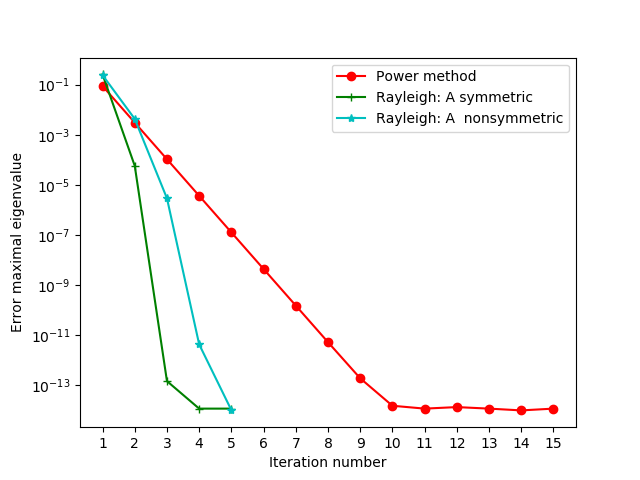
\includegraphics[scale=0.8]{../task2/task2.png}
\caption{Comparison of eigenvalues after $m$ iterations.}
\label{fig:task2}
\end{figure}

The Rayleigh quotient only uses the symmetric part of $A$ in
\begin{equation*}
  r(\mathbf{x}) = \mathbf{x}^{H}A\mathbf{x}
\end{equation*}
assuming $\mathbf{x}$ is normalized.
For $a_{13} = 4$ the matrix $A$ is no longer symmetric, i.e. $A\neq A^{H}$, but any square matrix can be decomposed into a symmetric part $A_{s}$ and a nonsymmetric part $A_{ns}$ by
\begin{equation}
  A = \underbrace{\frac{1}{2}\left(A + A^{H}\right)}_{= A_{s}} + \underbrace{\frac{1}{2}\left(A - A^{H}\right)}_{=A_{ns}}.
\end{equation}
Thus
\begin{equation*}
  r(\mathbf{x}) = \mathbf{x}^{H}A_{s}\mathbf{x} + \mathbf{x}^{H}A_{ns}\mathbf{x} = \mathbf{x}^{H}A_{s}\mathbf{x}
\end{equation*}
since
\begin{equation*}
 \mathbf{x}^{H}A_{ns}\mathbf{x}=\mathbf{x}^{H}A\mathbf{x} - \mathbf{x}^{H}A^{H}\mathbf{x} = 0.
\end{equation*}
For a nonsymmetric matrix all available information is not used.
